% !TeX encoding=utf8
% !TeX spellcheck = de_DE
% !TeX root = ../Diploma.tex

\chapter{Konzept des Servers}\label{sec:conceptServer}
Inhalt dieses Kapitels ist die Konzeption des RESTful Schachservers, welche die Grundlage für die Umsetzung selbigem bildet. Dabei dient der erste Abschnitt zur Erläuterung der Anforderungen, welche der Server mitbringen bzw. erfüllen soll. Enthalten ist dabei auch eine Erläuterung der benötigten Ressourcen. Der zweite Abschnitt dieses Kapitels befasst sich anschließend damit, wie der Zugriff auf einzelne Ressourcen des \gls{REST}-Servers erfolgen soll. Dabei werden alle möglichen Request-Methoden für die jeweiligen Ressourcen näher beleuchtet. Abschließend wird erläutert, wie das Designkonzept HATEOAS in dieser Anwendung erreicht werden kann.

\section{Anforderungen}\label{sec:anforderungen}
Die Grundanforderungen an den RESTful Schachserver sollen in erster Linie die Bereitstellung aller benötigten Ressourcen sein. Dabei sollen Elemente erstellt, ggf. bearbeitet und gelöscht werden können. Zusätzlich soll die Möglichkeit bestehen, einzelne oder alle gespeicherten Elemente eines Ressourcentyps abzufragen. Beim Erstellen eines neuen Ressourcenelements soll dieses in einer Datenbank gespeichert und die ID automatisch durch die Datenbank generiert werden.\\
\\
Um ein Schachspiel abzubilden, bedarf es dabei der Ressourcen Player (Spieler), Match (Partie) und Draw (Zug), welche in den nachfolgenden \hyperref[sec:resplayer, sec:resdraw]{Unterabschnitten~\ref{sec:resplayer} bis \ref{sec:resdraw}} näher betrachtet werden.\\
\\
Als abschließende Anforderung ist noch die Fehlertoleranz zu erwähnen. Denn die im Rahmen dieser Arbeit entstandene Praktikumsaufgabe\footnote{siehe \hyperref[chap:Appendix:A]{Anhang~\ref{chap:Appendix:A}}} soll durch zukünftige Studenten bearbeitet werden, wobei der Server als Grundlage dienen soll.

\subsection{Ressource: Player (Spieler)}\label{sec:resplayer}
Neben der ID, welche schon im Abschnitt \ref{sec:anforderungen} erwähnt wurde und durch die Datenbank generiert werden soll, muss der Player noch Informationen über seinen Namen und sein Passwort besitzen.\\
\\
Nach dem Anlegen eines neuen Players soll eine Änderung des Passwortes möglich, aber die des Namens nicht möglich sein.

\subsection{Ressource: Match (Partie)}\label{sec:resmatch}
Neben der ID muss ein Match Informationen über die beiden Spielteilnehmer und deren Figurenstellung auf dem Schachbrett besitzen. Zusätzlich soll registriert werden, welcher der beiden Player als nächstes seinen Zug tätigen muss, welche Möglichkeiten zum rochieren bestehen, ob ein Schlag \enquote{en passant} möglich ist und wenn ja auf welches Feld gezogen werden muss und wie viele Halbzüge gespielt wurden. Der Wert der Halbzüge soll dabei zurückgesetzt werden, sobald eine Bauernfigur gezogen oder eine beliebige Figur geschmissen wurde. Zusätzlich muss über ein Match ermittelt werden können, ob ein Spieler im Schach steht oder ob das Spiel schon bis zum Schachmatt gespielt wurde. All diese Informationen sollen zusätzlich noch als String in der \gls{FEN}\footnote{\label{foot:chapter}siehe \hyperref[sec:chessNotation]{Kapitel~\ref{sec:chessNotation}}} gespeichert werden.

\subsection{Ressource: Draw (Zug)}\label{sec:resdraw}
Die Ressource Draw muss zusätzlich zur ID noch weitere Informationen speichern, unter anderem die Farbe des Spielers, die Art der Spielfigur, Start- und Endfeld des Zuges, ob eine Figur geschlagen wurde, wenn ja ob durch \enquote{en passant} und ob seitens der Dame oder des König rochiert wurde. Diese Informationen sollen als String in der \gls{SAN}\footref{foot:chapter} gespeichert werden.

\section{Klassendiagramm}
Auf der Grundlage der im \hyperref[sec:anforderungen]{Kapitel~\ref{sec:anforderungen}} definierten Anforderungen wurde das \gls{UML} Klassendiagramm aus der \hyperref[fig:classdiagram]{Abbildung~\ref{fig:classdiagram}} entworfen. Neben den Klassen für die Repräsentation der Ressourcen aus den \hyperref[sec:resplayer, sec:resdraw]{Kapiteln~\ref{sec:resplayer} bis \ref{sec:resdraw}}, wurden noch weitere Hilfsklassen definiert, um die Grundstruktur feiner zu kapseln.\\
\\
Die Klasse \code{Field} dient dabei als Objekt zur Repräsentation eine Feldes auf dem Schachbrett, die Klasse \code{PieceSet} als Datencontainer der Figuren eines Players und die Klasse \code{Piece} als Darstellung einer einzelnen Figur. Die Enumerations \code{PieceType} und \code{PieceColor} dienen zur Bestimmung der Art und der Farbe einer Figur, wobei letztere auch zur Identifikation für Player bezogenen Daten genutzt wird. Die verbleibenden Klassen \code{PlayerHashMap}, \code{MatchHashMap}, \code{DrawList} und \code{PieceSetHashMap} dienen als Wrapper-Klassen zur besseren Repräsentation und werden nur für die Rückgabe von Ressourcenlisten verwendet.
\begin{sidewaysfigure}
	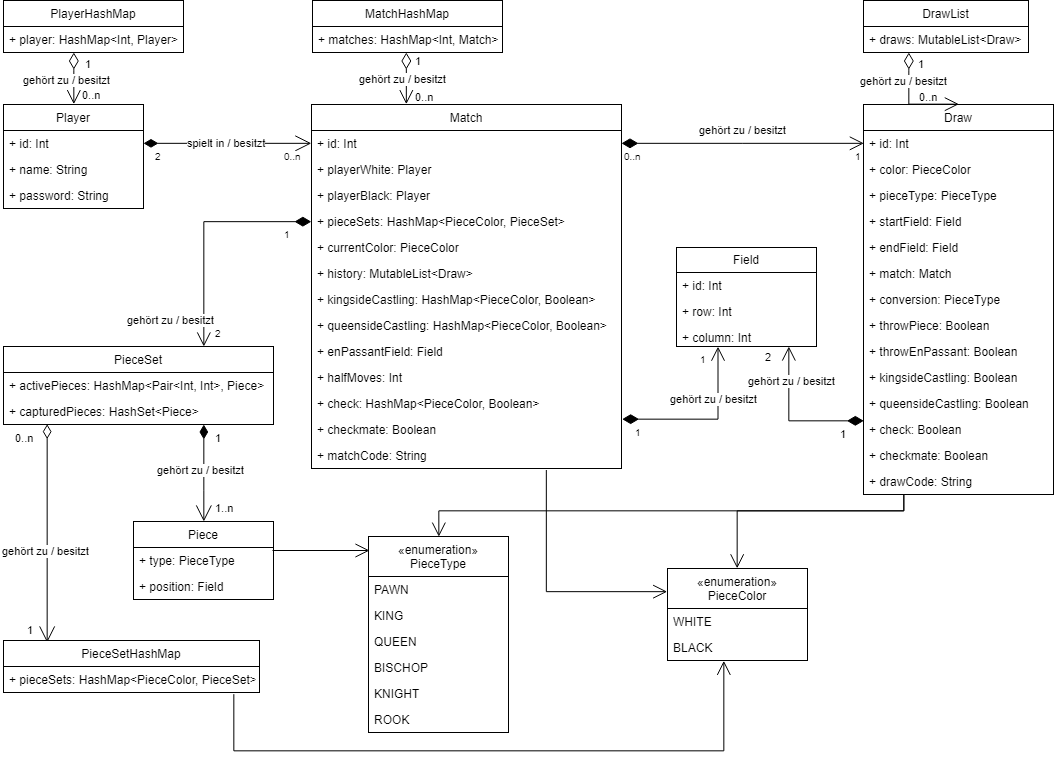
\includegraphics[width=0.9\textwidth]{images/classdiagram.png}
	\caption{Klassendiagramm: Modelle des Servers}
	\label{fig:classdiagram}
\end{sidewaysfigure}

\section{Ressourcenzugriffe mithilfe von Controllern}\label{sec:controller}
Die einzelnen Zugriffe auf die Ressourcen werden in den \hyperref[sec:rootController, sec:errorController]{Kapiteln~\ref{sec:rootController} bis \ref{sec:errorController}} nach ihrer Art bzw. deren Aufgaben einzelnen Controllern zugeordnet, um eine gute Übersicht zu wahren. Für alle Einstiegspunkte der \gls{REST}-\gls{API} wird die Request-Methode \code{OPTIONS} bereitgestellt, über die ermittelt werden kann, welche Methoden für den jeweiligen Einstiegspunkt zur Verfügung stehen.\\
\\
Etwaige Requestparameter können in den Formaten \gls{JSON} oder x-www-form-urlencode an den Request übergeben werden. Gesendeten Anfragen liefern anschließend ihr Feedback je nach Wunsch des Clients, via Content Negotiation, entweder in \gls{JSON} oder als \gls{XML} zurück. Dafür werden drei Strategien zur Umsetzung bereitgestellt, entweder mittels Suffix, einem URL-Parameter oder dem \gls{HTTP} Accept-Header. 

\subsection{Root Controller}\label{sec:rootController}
Mit dem Root Controller wird der Einstiegspunkt an der \gls{URI} \path{/api} bereitgestellt. Ein GET-Request an diesem Einstiegspunkt liefert aber ausschließlich Links zu den einzelnen Startpunkten der Ressourcen Player, Match und Draw. Dies wiederum dient der Umsetzung des Konzeptes HATEOAS, welches im \hyperref[sec:konzeptHATEOAS]{Kapitel~\ref{sec:konzeptHATEOAS}} genauer definiert wird und ausführlichere Erläuterungen enthält, wie das Ziel dieses Konzeptes erreicht werden kann.\\
\\
Die nachfolgende \hyperref[fig:rootController]{Abbildung~\ref{fig:rootController}} dient dabei als Veranschaulichung des Einstiegspunktes.\\
\begin{figure}[htb]
	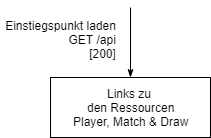
\includegraphics[width=0.323\textwidth]{images/root-controller.png}
	\caption{Root Controller - Übersicht der Einstiegspunkte}
	\label{fig:rootController}
\end{figure}

\subsection{Player Controller}\label{sec:playerController}
Der Player Controller stellt zwei Einstiegspunkte an den \glspl{URI} \path{/api/players} und \path{/api/players/{id}} zur Verfügung bereit. Der Parameter \path{{id}} dient dabei als Platzhalter für die ID eines Players.\\
\\
Am ersten Einstiegspunkt wird eine Liste aller Spieler über einen GET-Request bereitgestellt. Des Weiteren besteht an diesem die Möglichkeit, einen neuen Player mithilfe eines POST-Requests zu erzeugen. Dabei muss als Parameter der Name und das Passwort des Players mitgegeben werden. Die ID wird durch die Datenbank mittels Autoinkrement erzeugt. Bei erfolgreicher Erstellung des Players wird dieser als \gls{HTTP}-Response zurückgegeben. Tritt bei diesem Prozess jedoch ein Fehler, wird stattdessen dieser zurückgegeben.\\
\\
Am zweiten Einstiegspunkt wird ein einzelner existierender Player über einen GET-Request bereitgestellt, über einen DELETE-Request gelöscht und über einen PATCH-Request aktualisiert. Dabei wird bei einer Aktualisierung eines Players nur das Passwort, laut Anforderungen\footnote{siehe \hyperref[sec:anforderungen]{Kapitel~\ref{sec:anforderungen}}}, geändert.\\
\\
Für ein besseres Verständnis der einzelnen Einstiegspunkte, mit den dazugehörigen Request-Methoden, bietet die \hyperref[fig:playerController]{Abbildung~\ref{fig:playerController}} eine visuelle Verdeutlichung des Player Controllers.\\
\begin{figure}[htb]
	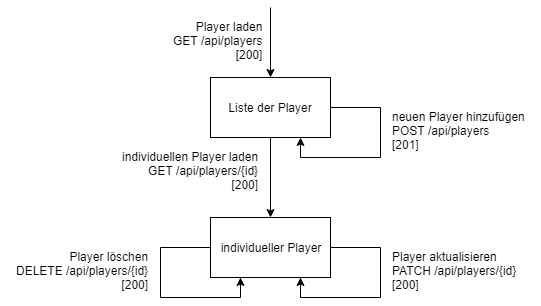
\includegraphics[width=0.816\textwidth]{images/player-controller.png}
	\caption{Player Controller - Übersicht der Einstiegspunkte}
	\label{fig:playerController}
\end{figure}

\subsection{Match Controller}\label{sec:matchController}
Die \glspl{URI} \path{/api/matches}, \path{/api/matches/{id}}, \path{/api/matches/{id}/draws} und \path{/api/matches/{id}/pieceSets} werden durch den Match Controller bereitgestellt.\\
\\
Dabei dient die erste \gls{URI} ebenso wie beim Player Controller der Zurverfügungstellung einer Liste aller registrierten Matches und dem Anlegen neuer. Das Bereitstellen der Liste erfolgt mittels GET- und das Anlegen mittels POST-Request. Der GET-Request stellt dabei zwei optionale boolesche Parameter \code{includeHistory} und \code{includePieceSets} bereit, womit das Senden der Historie von Draws bzw. der Figurenstellung bestimmt wird. Dabei besitzen die beiden Parameter standardmäßig den Wert \code{true}. Um ein neues Match zu registrieren, müssen dabei die ID's der beiden Spielteilnehmer als Parameter mitgesendet werden. Anhand des Parameternamens wird festgelegt, welcher Spieler Weiß und welcher Schwarz spielt.\\
\\
Der zweite Einstiegspunkt in diesem Controller wird ausschließlich dazu verwendet, um einzelne Matches mithilfe eines GET-Request anzufordern oder mit einem DELETE-Request zu löschen. Für das Anfordern eines einzelnen Matches stehen dabei, ebenso wie beim Request einer Match-Liste, die zwei optionalen booleschen Parameter \code{includeHistory} und \code{includePieceSets} bereit. Sollte ein Nutzer ein Match löschen, so werden die zugehörigen Draws automatisch mit gelöscht. Um eine unrechtmäßige Manipulation der Match-Daten durch einen Nutzer zu verhindern, steht keine Möglichkeit bereit, ein Match direkt zu aktualisieren. Änderungen der Match-Daten erfolgen ausschließlich über das Hinzufügen von neuen Draws\footnote{siehe \hyperref[sec:drawController]{Kapitel~\ref{sec:drawController}}}.\\
\\
Die letzten beiden Einstiegspunkte dienen dazu, große Match bezogene Daten separat zu ermitteln. Dabei wird mittels GET-Request an der \gls{URI} \path{/api/matches/{id}/draws} eine Liste aller Draws und über die \gls{URI} \path{/api/matches/{id}/pieceSets} eine Map mit allen Figuren der beiden Spielteilnehmer bereitgestellt. Neben den aktuell auf dem Spielfeld stehenden Figuren werden dabei auch die Daten der bereits Geschmissenen mitgeschickt.\\
\\
Die \hyperref[fig:matchController]{Abbildung~\ref{fig:matchController}} bietet für die zuvor definierten Einstiegspunkte eine grafische Veranschaulichung.\\
\begin{figure}[htb]
	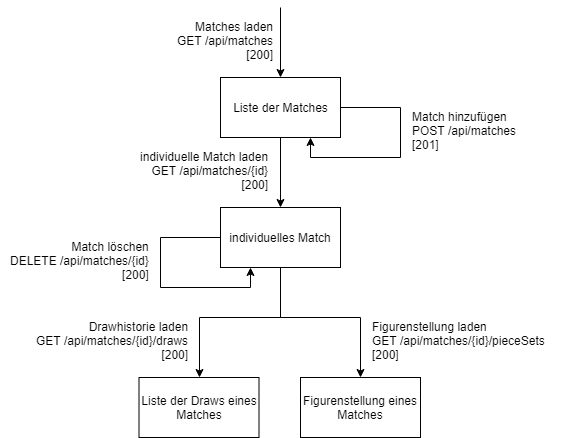
\includegraphics[width=0.85\textwidth]{images/match-controller.png}
	\caption{Match Controller - Übersicht der Einstiegspunkte}
	\label{fig:matchController}
\end{figure}

\subsection{Draw Controller}\label{sec:drawController}
Der Draw Controller stellt drei Einstiegspunkte an den \glspl{URI} \path{/api/draws}, \path{/api/draws/{id}} und \path{/api/draws/ai} bereit. \\
\\
Am ersten Einstiegspunkt wird dabei wieder eine Liste mittels GET- und das Hinzufügen mittels POST-Request von Draws zur Verfügung gestellt. Für das Hinzufügen eines neuen Draws ist die ID des Matches und der Draw-Code in der \gls{SAN} als Parameter notwendig. Zusätzlich besteht die Möglichkeit, die Zeilen- und Spaltennummer der Startposition mitzugeben. Wenn diese Informationen nicht mitgegeben werden, wird die Startposition vom Controller kalkuliert. Spalten sind dabei als Nummern und nicht als Buchstaben zu übergeben\footnote{A $\rightarrow$ 1; B $\rightarrow$ 2; C $\rightarrow$ 3; D $\rightarrow$ 4; E $\rightarrow$ 5; F $\rightarrow$ 6; G $\rightarrow$ 7; H $\rightarrow$ 8}. Nach erfolgreicher Validierung des Draw-Codes wird der Draw dem zugehörigen Match hinzugefügt und die Match-Daten aktualisiert.\\
\\
Über den zweiten Einstiegspunkt ist die Abfrage nach einem einzelnen Draw möglich, aber eine Löschung oder Aktualisierung nicht. Sonst wäre eine Manipulation der Match-Daten seitens des Nutzers möglich. Die Entfernung von Draws erfolgt ausschließlich über die Löschung des dazugehörigen Matches\footnote{siehe \hyperref[sec:matchController]{Kapitel~\ref{sec:matchController}}}.\\
\\
Der dritte Einstiegspunkt stellt mittels POST-Request die Möglichkeit bereit, einen Draw, mithilfe einer künstlichen Intelligenz, zu einem Match hinzuzufügen. Dafür muss ausschließlich die ID des benötigten Matches als Request-Parameter mitgegeben werden.\\
\\
Wie in den vorherigen Kapiteln bietet die \hyperref[fig:drawController]{Abbildung~\ref{fig:drawController}} ein Veranschaulichung der definierten Einstiegspunkte.\\
\begin{figure}[htb]
	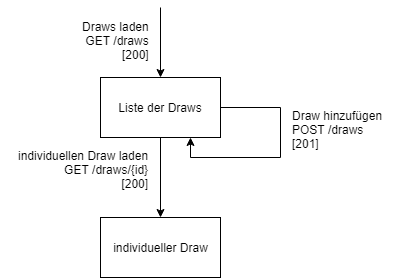
\includegraphics[width=0.7735\textwidth]{images/draw-controller.png}
	\caption{Draw Controller - Übersicht der Einstiegspunkte}
	\label{fig:drawController}
\end{figure}

\subsection{Error Controller}\label{sec:errorController}
Mithilfe des Error Controllers wird gewährleistet, dass alle nicht in der \gls{REST}-\gls{API} definierten Einstiegspunkte bzw. nicht definierte Request-Methoden an den Einstiegspunkten abgefangen werden. Tritt ein solcher Fall auf, so wird ein Fehler vom Server zurückgegeben. Somit wird verhindert, dass ein Nutzer der \gls{API} einen Serverfehler, mit dem HTTP-Statuscode \code{500 Internal Server Error}\footnote{siehe \cite[A.2.5]{kretzschmar}}, zurückerhält.

\section{Erreichung des Designkonzepts HATEOAS}\label{sec:konzeptHATEOAS}
Um das Ziel der Selbstbeschreibung, welches das Konzept HATEOAS verfolgt, zu erreichen, gibt es mehrere Lösungswege.\\
\\
Zum einen besteht die Möglichkeit der Erweiterung einer Ressource, wodurch diese als Hypermedia Format angesehen werden kann. Ein Beispiel dafür ist die \gls{HAL}, welche in der Spezifikation \cite{halSpezification} definiert wurde. Diese stellt mittels eines Dialektes von \gls{JSON} die \gls{MIME} Typen \code{application/hal+json} und \code{application/hal+xml} bereit, bei denen Ressourcen mit Relationen, in Form von Hyperlinks, ergänzt werden können.\\
\\
Eine weitere Lösungsvariante kann durch den Link-Header des \gls{HTTP}-Response realisiert werden. Diesem kann einfach eine Menge von Links in Form eines Strings übergeben werden, welchen der Client anschließend auswerten kann.\\
\\
Welche Variante die bessere ist, liegt im Auge des Betrachters. Für die Implementierung des Schach-Servers wurde Variante zwei gewählt, weil dadurch die Trennung der Links und der eigentlichen Ressource strikter wahrgenommen werden kann. Auch Kai Spichale bevorzugt diese Variante, denn dieser betrachtet die Links in seinem Buch \cite[158]{apiDesign} als Metainformationen und diese gehören seiner Meinung nach nicht in die Ressource.